In this section we will reason and explain the experiments done with the algorithm to demonstrate the good performance and efficiency of the algorithm. The experiments were replicated from the paper. Six main experiments were performed, 3 with artificial datasets and 3 with real datasets.

The artificial datasets will be created using the Artificial Dataset Generator class mentioned in the previous section. The number of gausssians will be set to the same number of clusters to be detected in the clustering algorithms and the standard deviation will be set to ensure an overlap of around 5\%. For the real dataset, we will use the gas-sensor dataset \cite{UCIGas} from the UCI repository \cite{UCI}, particularly the ethylene\_methane dataset which contains 4178504 instances and 16 features. In order to construct the dataset of the wanted size, a random number of instances will be selected and a random number of features will be selected as well acording to the parameters $K$ and $D$ that will be set in each of the experiments.

Three main experiments were performed with each dataset: The computation of distances comparison experiment, the standard error experiment and finally the instance ratio experiment.

\section{Distance computation}

The first experiment done was the distance comparison experiment. RPKM was evaluated against scikit-learn's KMeans initialized with the k-means++ algorithm and scikit-learn's MiniBatchKMeans with batch sizes of $b \in \{100, 500, 1000\}$. The RPKM algorithm was evaluated for $m \in [1\dots6]$. This experiment was replicated for the artificial and real datasets. In the case of artificial dataset, the distance computation values were averaged over 10 replicas of the dataset, meaning that 10 random datasets with the same number of clusters K, number of dimensions D and number of instances N are generated and then their results are averaged. In the case of the real dataset, 10 replicas were used as well. In this case, a replica corresponds to a random selection of D features and N instances from the dataset.

In the case of the RPKM algorithm the number of distance computations are calculated as:
$$d_{RPKM} = \sum_{i=1}^m niter_i * |R_i| *K$$
Or in other words, the distance computations $nd$ at iteration $i$ are the number of iterations for the WL algorithm at that iteration $niter_i$ times the number of representatives $|R_i|$ at that iteration times the number of clusters $K$. Then the distance computations for all RPKM iterations are added.

For the KMeans algorithm, the number of distances are computed by the following expression:
$$d_{kmeans} = d_{init} + d_{lloyd}$$
$$d_{init} \bigg\rvert_{init=k-means++} = N * \sum_{i=1}^K i = \frac{K*(K+1)}{2} * N$$
$$d_{lloyd} = niter * K * N$$
Or in other words, the distance computations for the KMeans is the sum of the number of distances of the initialization and the number of instances of lloyd's algorithm. For the k-means++ inicialization, for each center to be created the algorithm computes the distances of the distances of the cluster centers already initialized, which at each iteration increases by 1 until reacing K clusters. this can be computed as the sum of all natural number until K times the dataset size $N$. The number of distance computations for the lloyd algorithm is defined as the number of iterations done until convergence times a $K$ * $N$ distance computation matrix that is computed each iteration to assign each instance to a cluster.

Finally, the MiniBatchKMeans algorithm follows a similar computation scheme as KMeans but the $d_{lloyd}$ is computed differently as it is performed with a batch size $b$.
$$d_{kmeans} = d_{init} + d_{lloyd}$$
$$d_{init} \bigg\rvert_{init=k-means++} = \frac{K*(K+1)}{2} * N$$
$$d_{lloyd} = niter * K * b$$
Where the only notable difference is that the distances computed in each iteration of the MiniBatchKMeans are not $K*N$ as in KMeans but rather $K*b$ due to the computation being done through batches.

Using this computation schemes, we perform a sweep for $K \in \{3, 9\}$, $D \in \{2, 4, 8\}$. For the artificial datasets, $N \in \{1e2, 1e3, 1e4, 1e5, 1e6\}$ while for the real dataset the values of N were chosen to be $N \in \{4000, 12000, 40000, 120000, 400000, 1200000, 4000000\}$ as in the paper. The results obtained with this experiment are shown in \ref{fig:distance_art} and \ref{fig:distance_real} containing the results for the artificial and real dataset respectively.

\begin{figure}[!ht]
    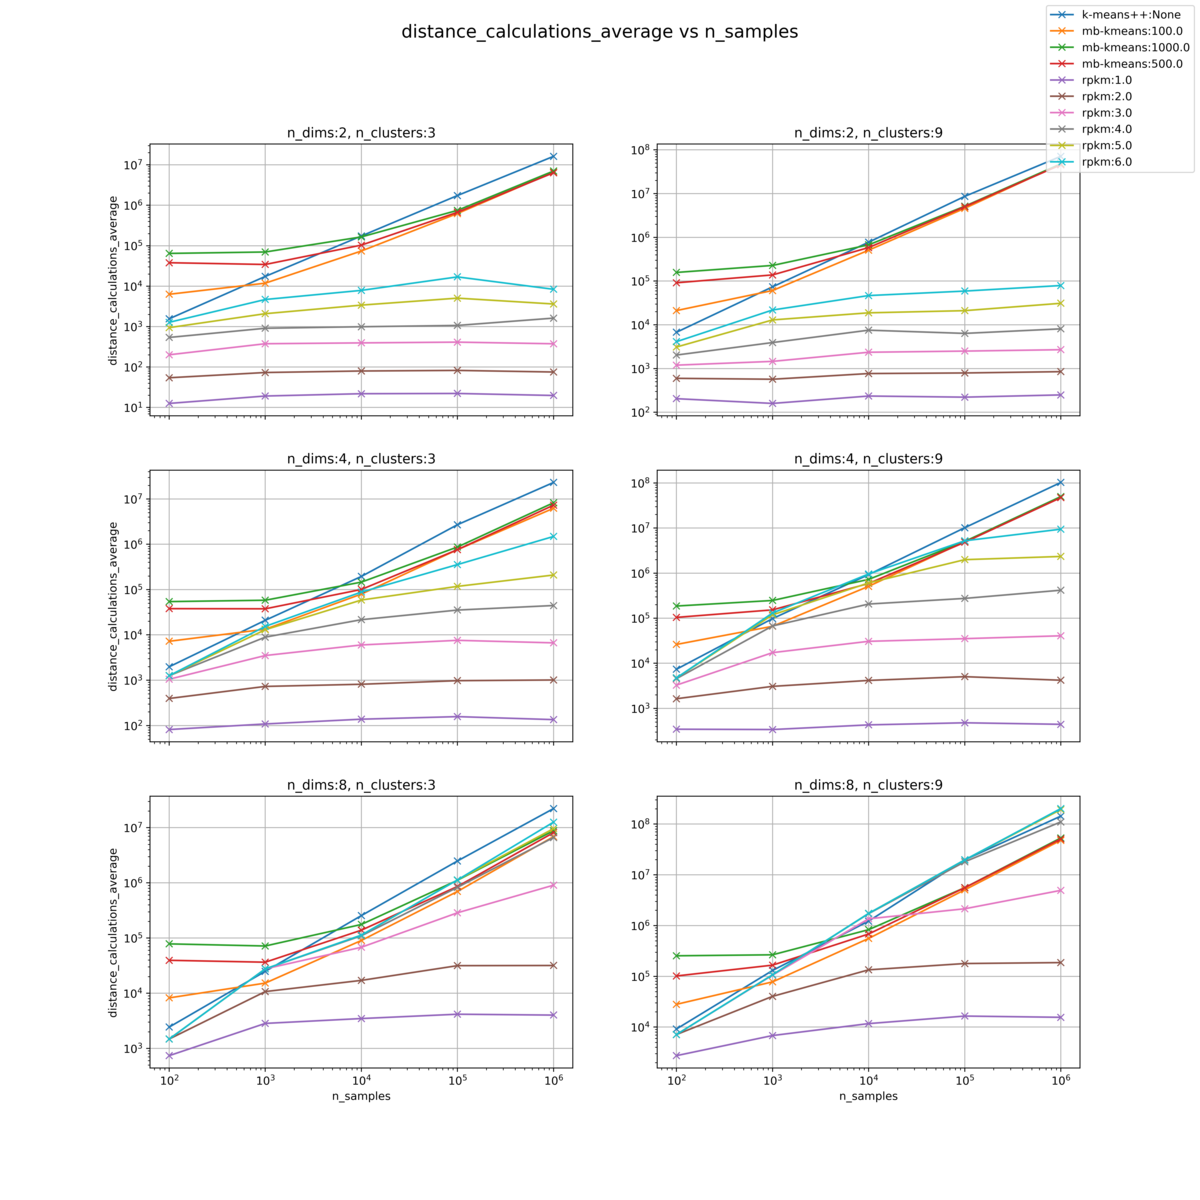
\includegraphics[width=\linewidth]{images/experiments/distances_artificial.png}
    \caption{Distance computation results in artificial datasets}
    \label{fig:distance_art}
\end{figure}
'
\begin{figure}[!ht]
    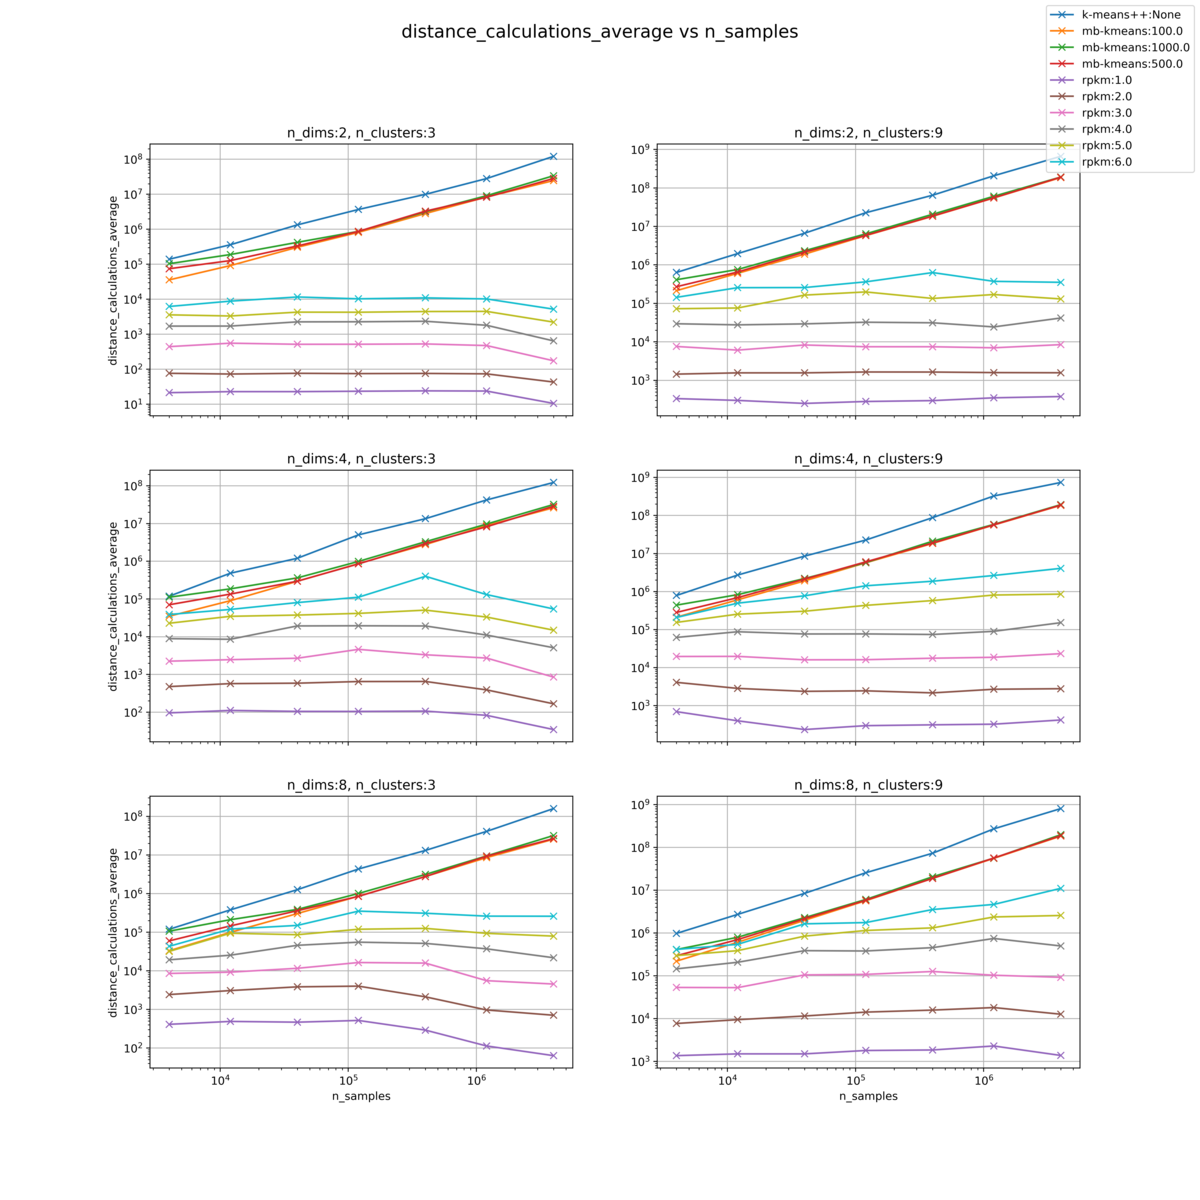
\includegraphics[width=\linewidth]{images/experiments/distances_real.png}
    \caption{Distance computation results in real datasets}
    \label{fig:distance_real}
\end{figure}

The figures show promising results where the number of distance computations is usually smaller than the number of computations for k-means++. In the artificial dataset's results we can see a little bit of overlap, especially in the case of D=8 and K=9, where all but the RPKM with $m \in \{1,2,3\}$ seem to have very similar performance. On the other hand, the real dataset's results show very promising results where none of the distance computations for any of the K, D combinations use more than the distances computed by MiniBatchKMeans and KMeans.

\section{Instance Ratio}

We define the instance ratio as the size of the partition divided by the number of instances in the dataset $|P|/n$. The goal of this experiment is to demonstrate the reduction of data points given to the WL algorithm at each iteration of the PRKM algorithm. In order to demonstrate the reduction, the artificial and real dataset were used like in the previous experiment. The number of replicas was set to 10, the number of instances $N$, the number of clusters $K$ and the number of dimensions $D$ were kept as the same as the previous experiment. In this experiment, only the RPKM algorithm was tested as it makes no sense to talk about partitions in KMeans and MiniBatchKMeans.

The instance ratio was computed for each max\_iter ($m$) value for the RPKM and extracted at the end of the fit stage as the number of subsets in the $m^{th}$ partition divided by the number of instances of the dataset. The results for the experiments can be seen in \ref{fig:instance_art} and \ref{fig:instance_real} containing the results for the artificial and real dataset respectively.

\begin{figure}[!ht]
    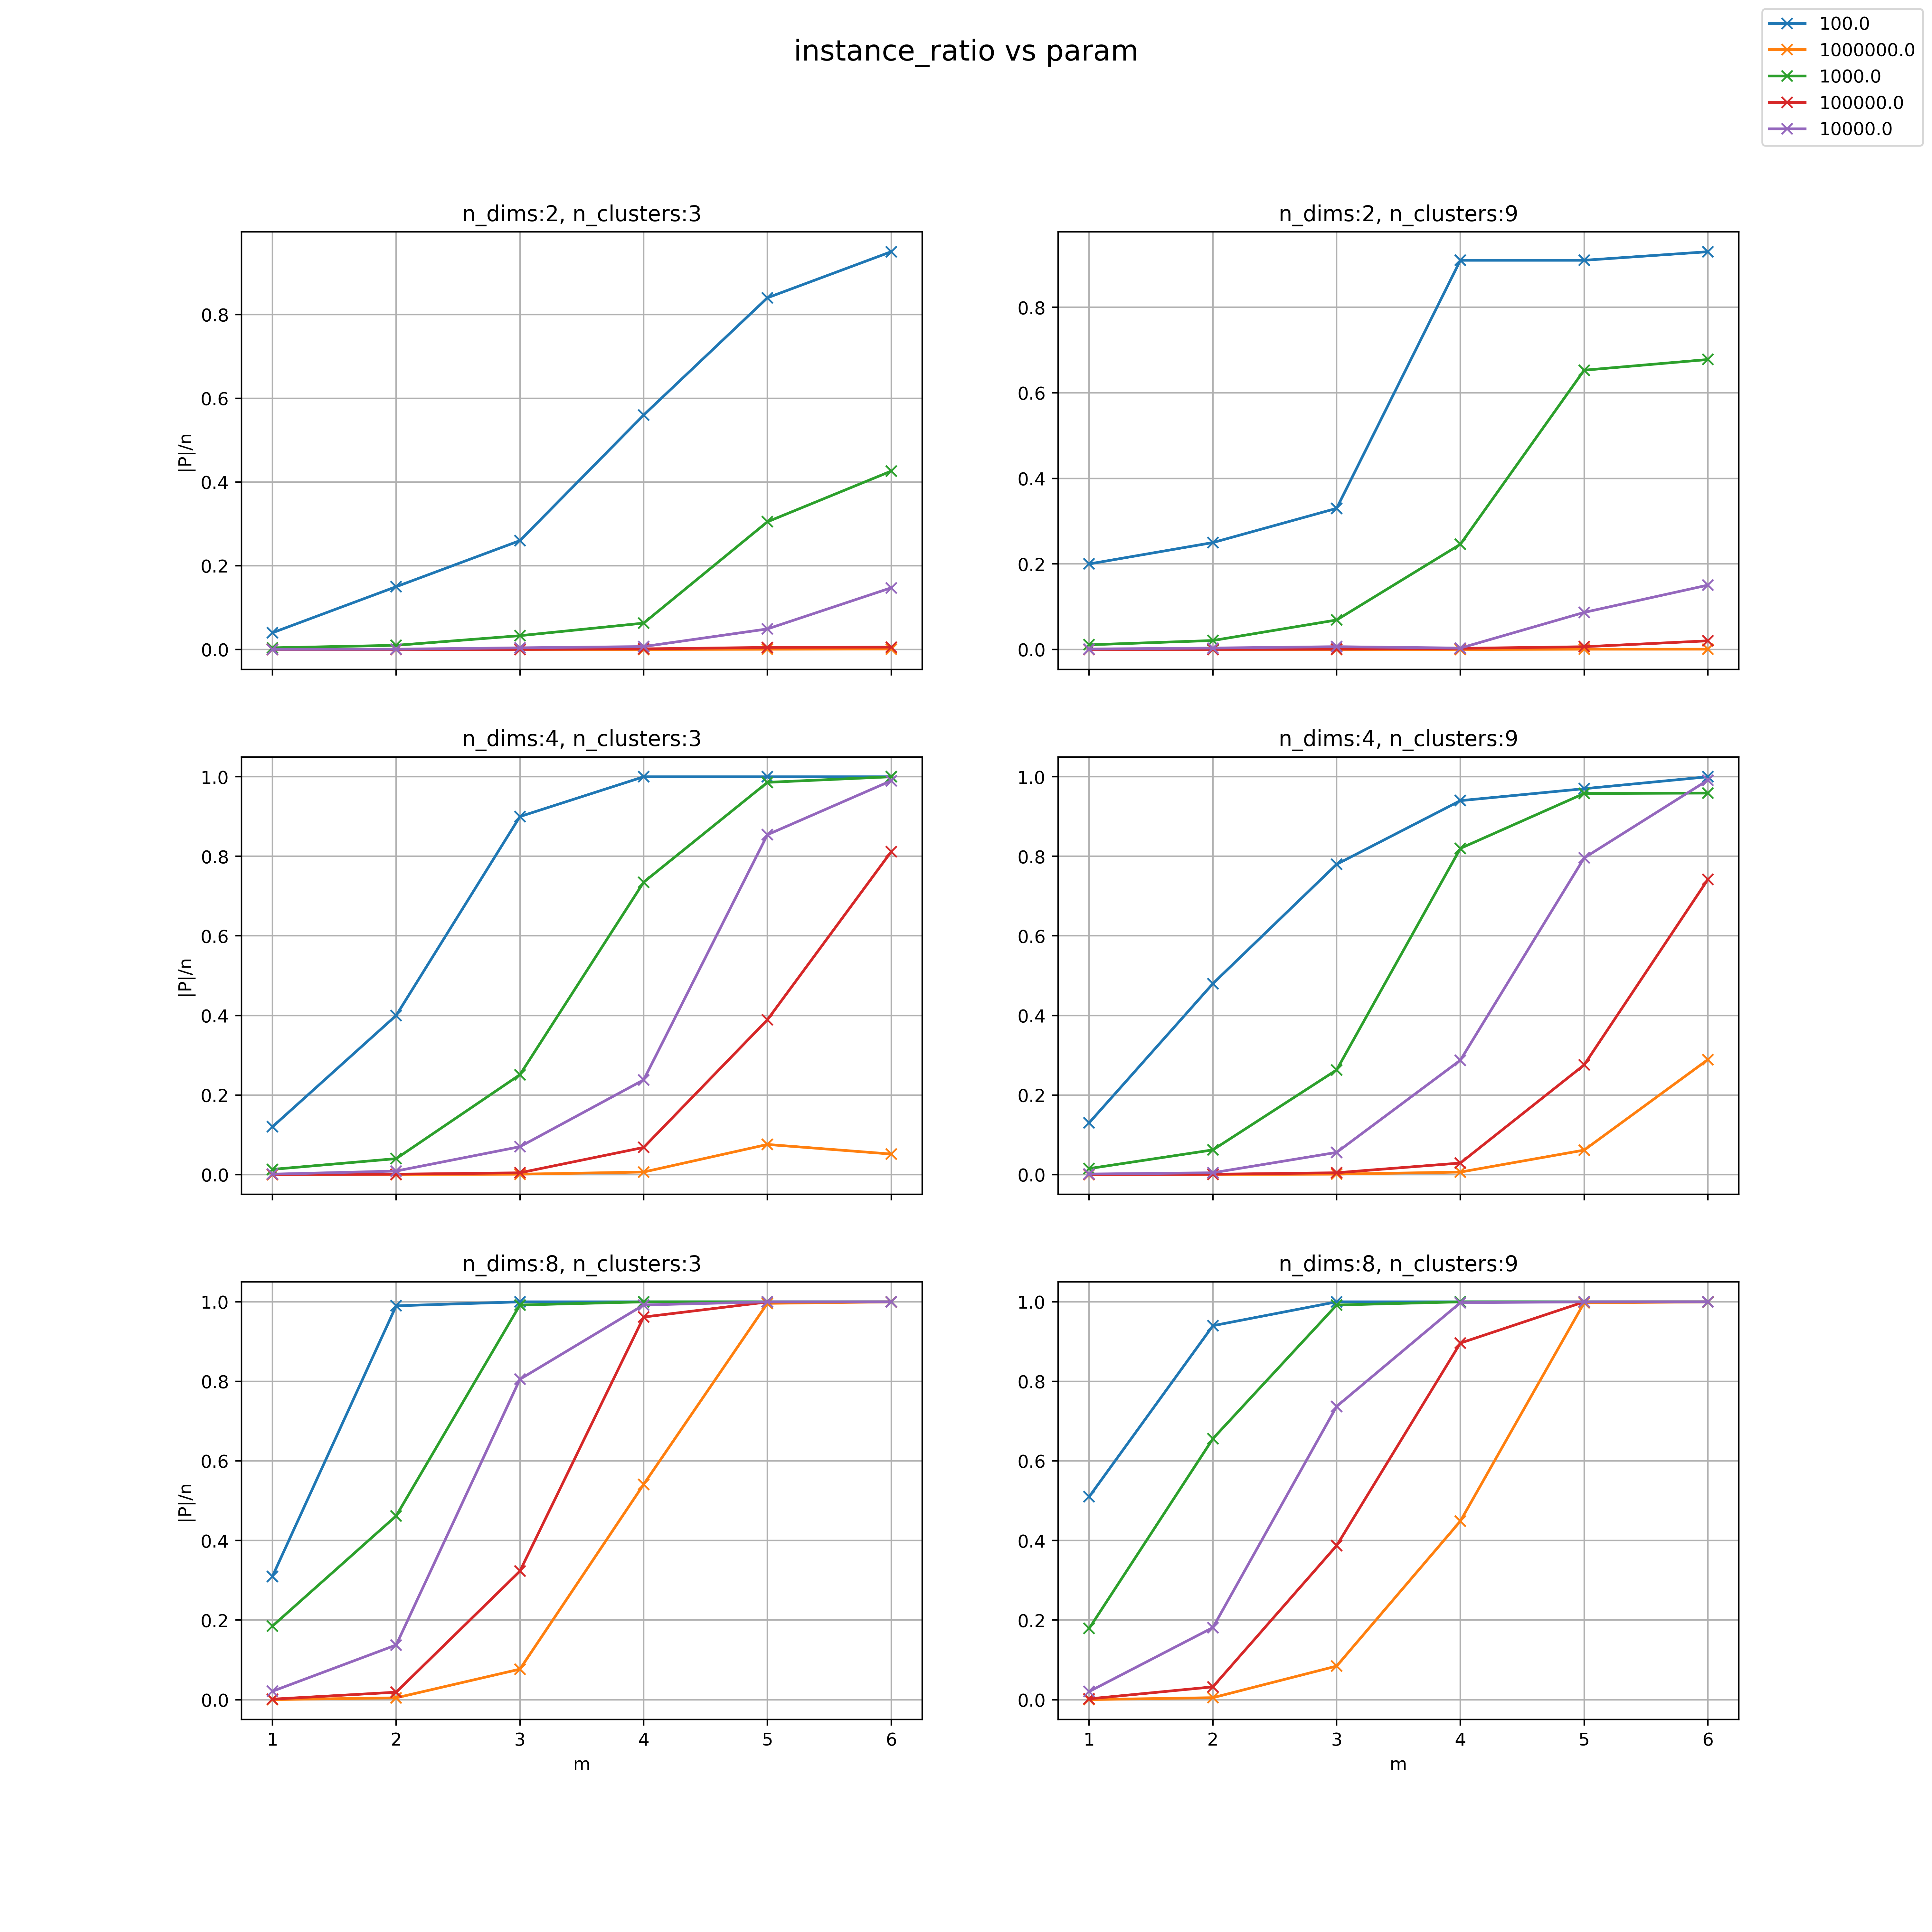
\includegraphics[width=\linewidth]{images/experiments/instance_ratio_artificial.png}
    \caption{Instance ratio computation results in artificial datasets}
    \label{fig:instance_art}
\end{figure}

\begin{figure}[!ht]
    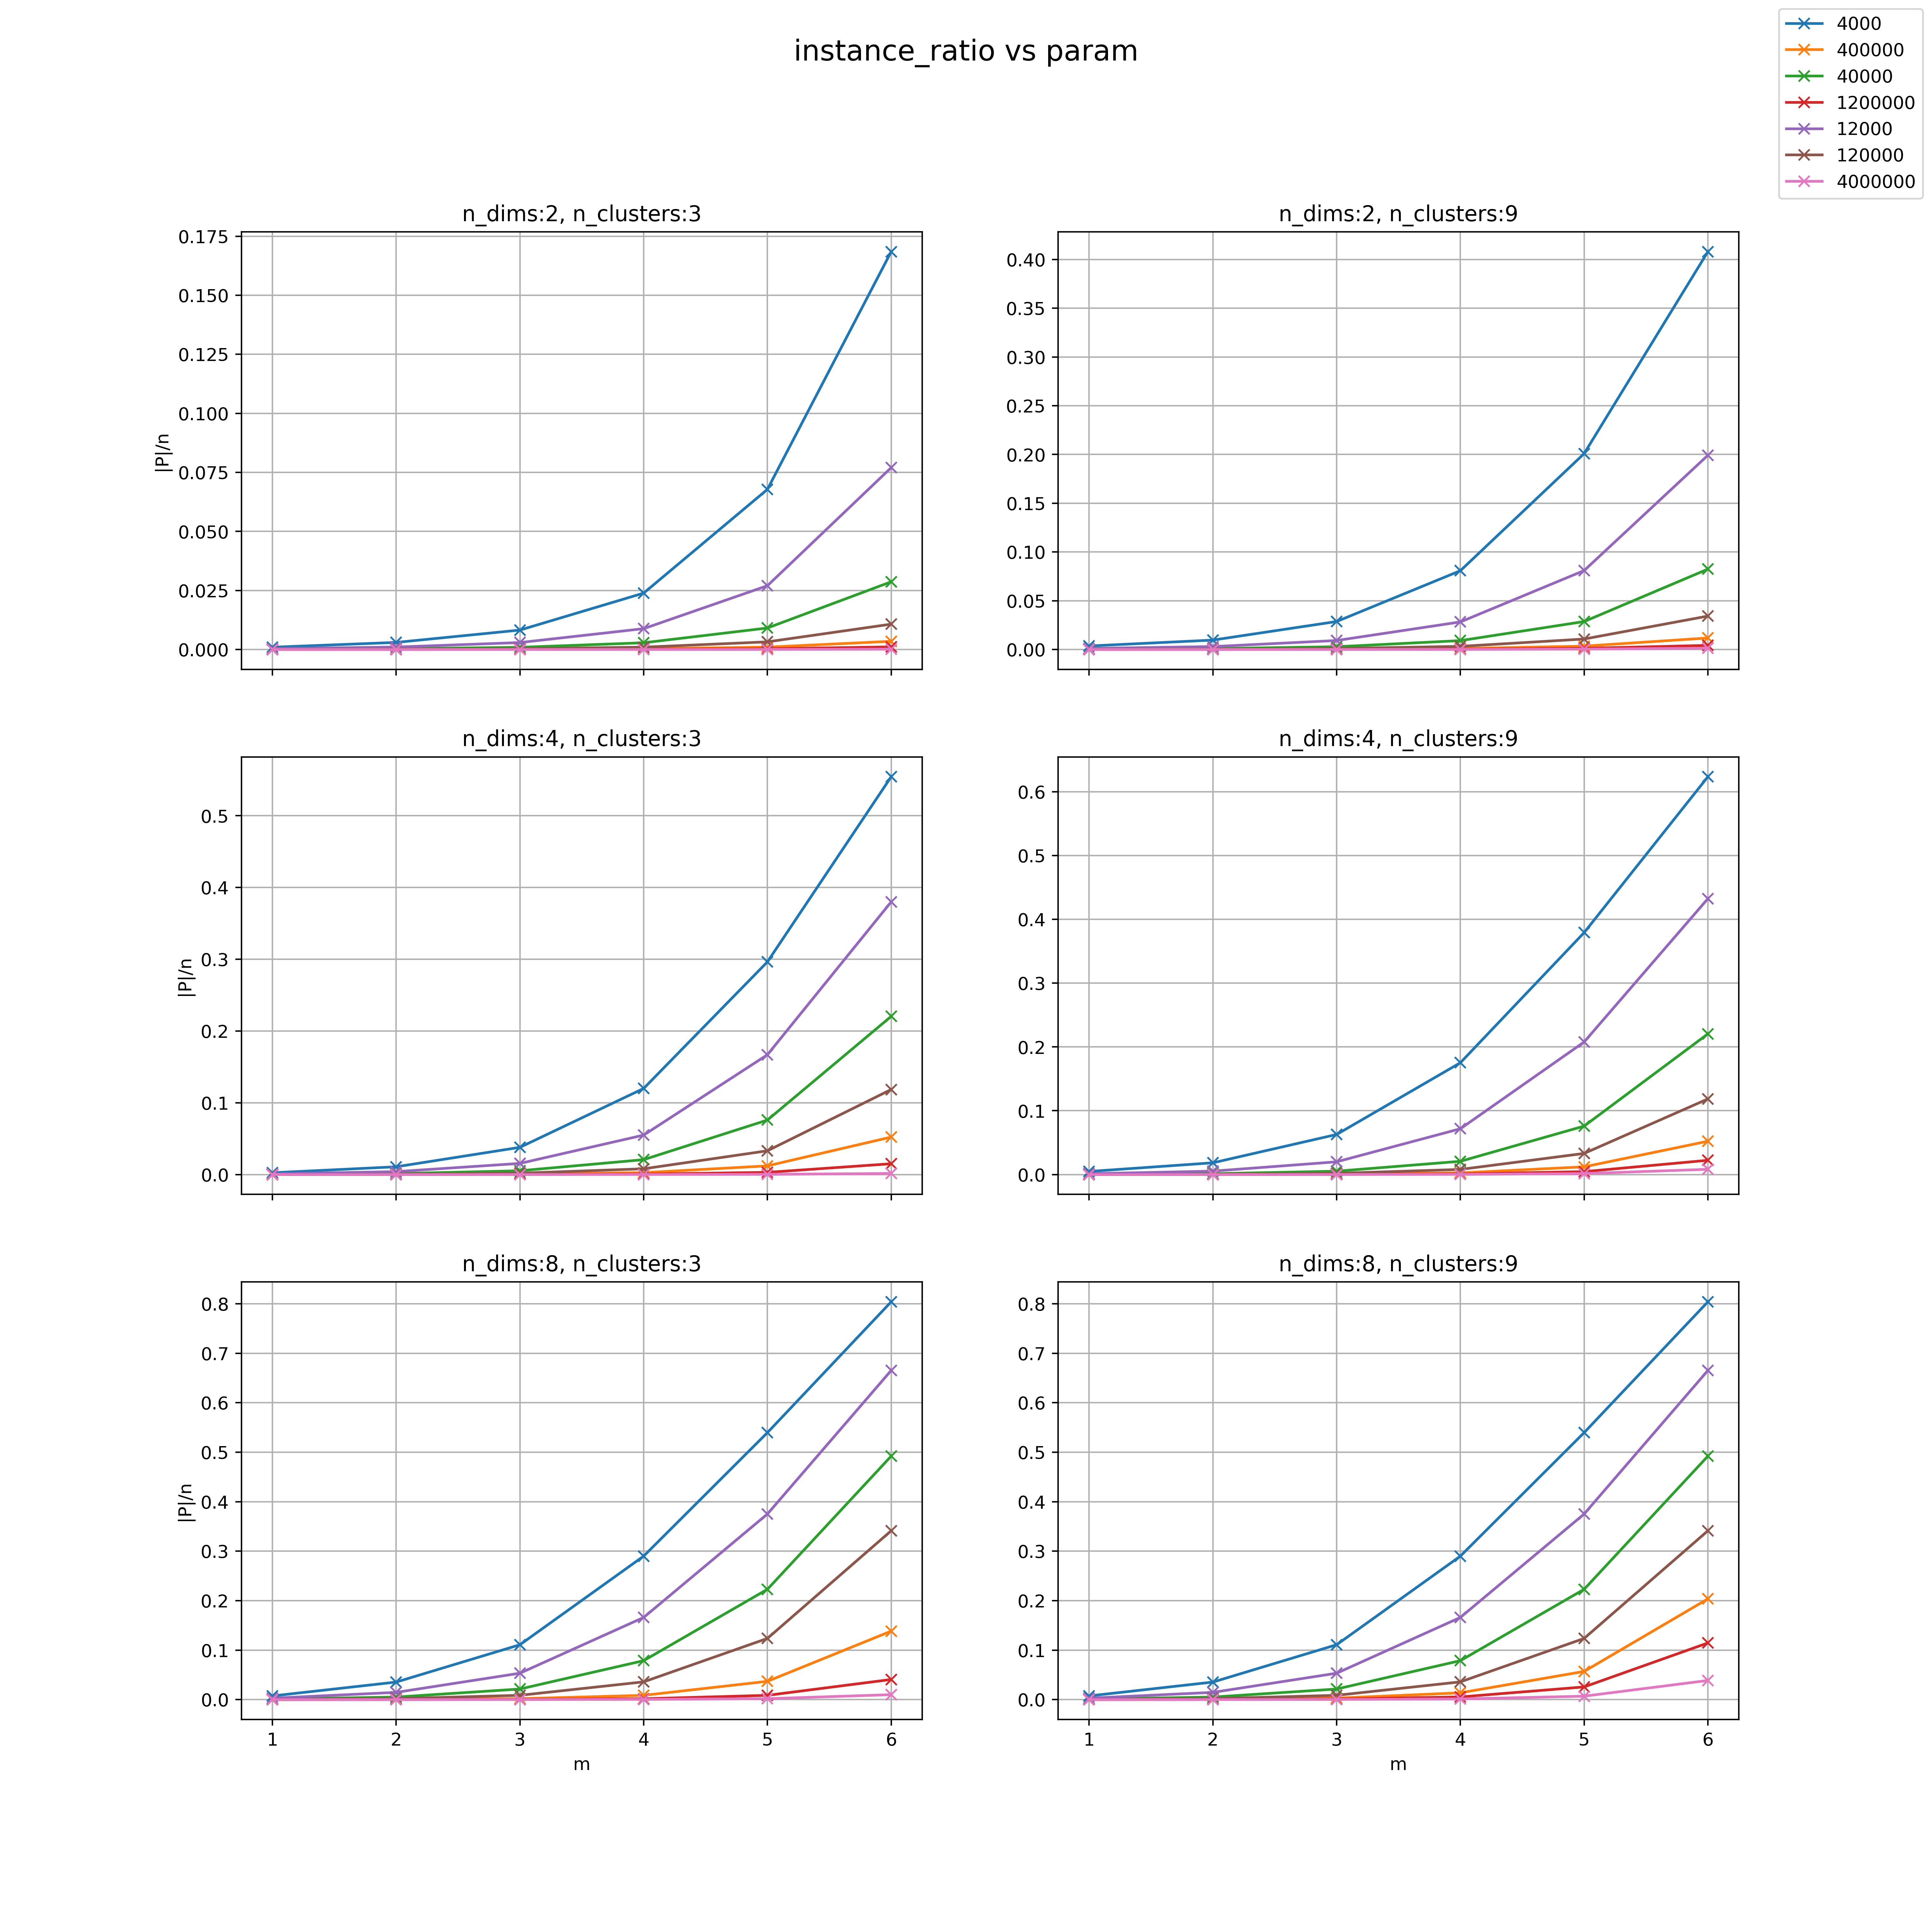
\includegraphics[width=\linewidth]{images/experiments/instance_ratio_real.png}
    \caption{Instance ratio computation results in real datasets}
    \label{fig:instance_real}
\end{figure}

In the figures we can appreciate that on the first iterations of the RPKM algorithm, the number of representatives (or subsets) is very small wrt. the number of samples in the dataset as is expected. The exponential growth of the number of subsets is very apparent in the real dataset's results but in the artificial dataset's results, it is less apreciable as it reaches a ratio closer to 1 very quickly compared to the real dataset. For smaller number of samples in the dataset it's quite more apparent that the ratio grows a lot quicker than in the datasets that have a considerable ammount of instances. The results are promising as the algorithm is ment to be used with large datasets, and it seems to use a very small number of instances. We can note as well that the ratio increases very quickly wrt to the number of dimensions, as the number of hypercubes is exponential wrt the number of dimensions and the number of partitions will be bigger.

\section{Quality of the approximation}

In this section we will discuss the standard error (std.error) metric proposed in the paper and the experiment realized to quantitatively analyze the difference between the clustering centers extracted with RPKM and the clusters extracted with a k-means++ algorithm. In the paper, they define the clustering error as:

$$E(C) = \sum_{x \in D} \min_{k=1,\dots,K}||x-c_k||^2$$

This expression will be used to compute the clustering error of the RPKM algorithm and the KMeans algorithm using the following expression:

$$\rho = \frac{E_{km++} - E_{RPKM}}{E_{km++}}$$

This will always yield $\rho < 0$ and the more negative the value of $\rho$ the worse is the approximation of the RPKM centers. The results for this experiment can be seen in \ref{fig:error_art} and \ref{fig:error_real} containing the results for the artificial and real datasets respectively.

\begin{figure}[!ht]
    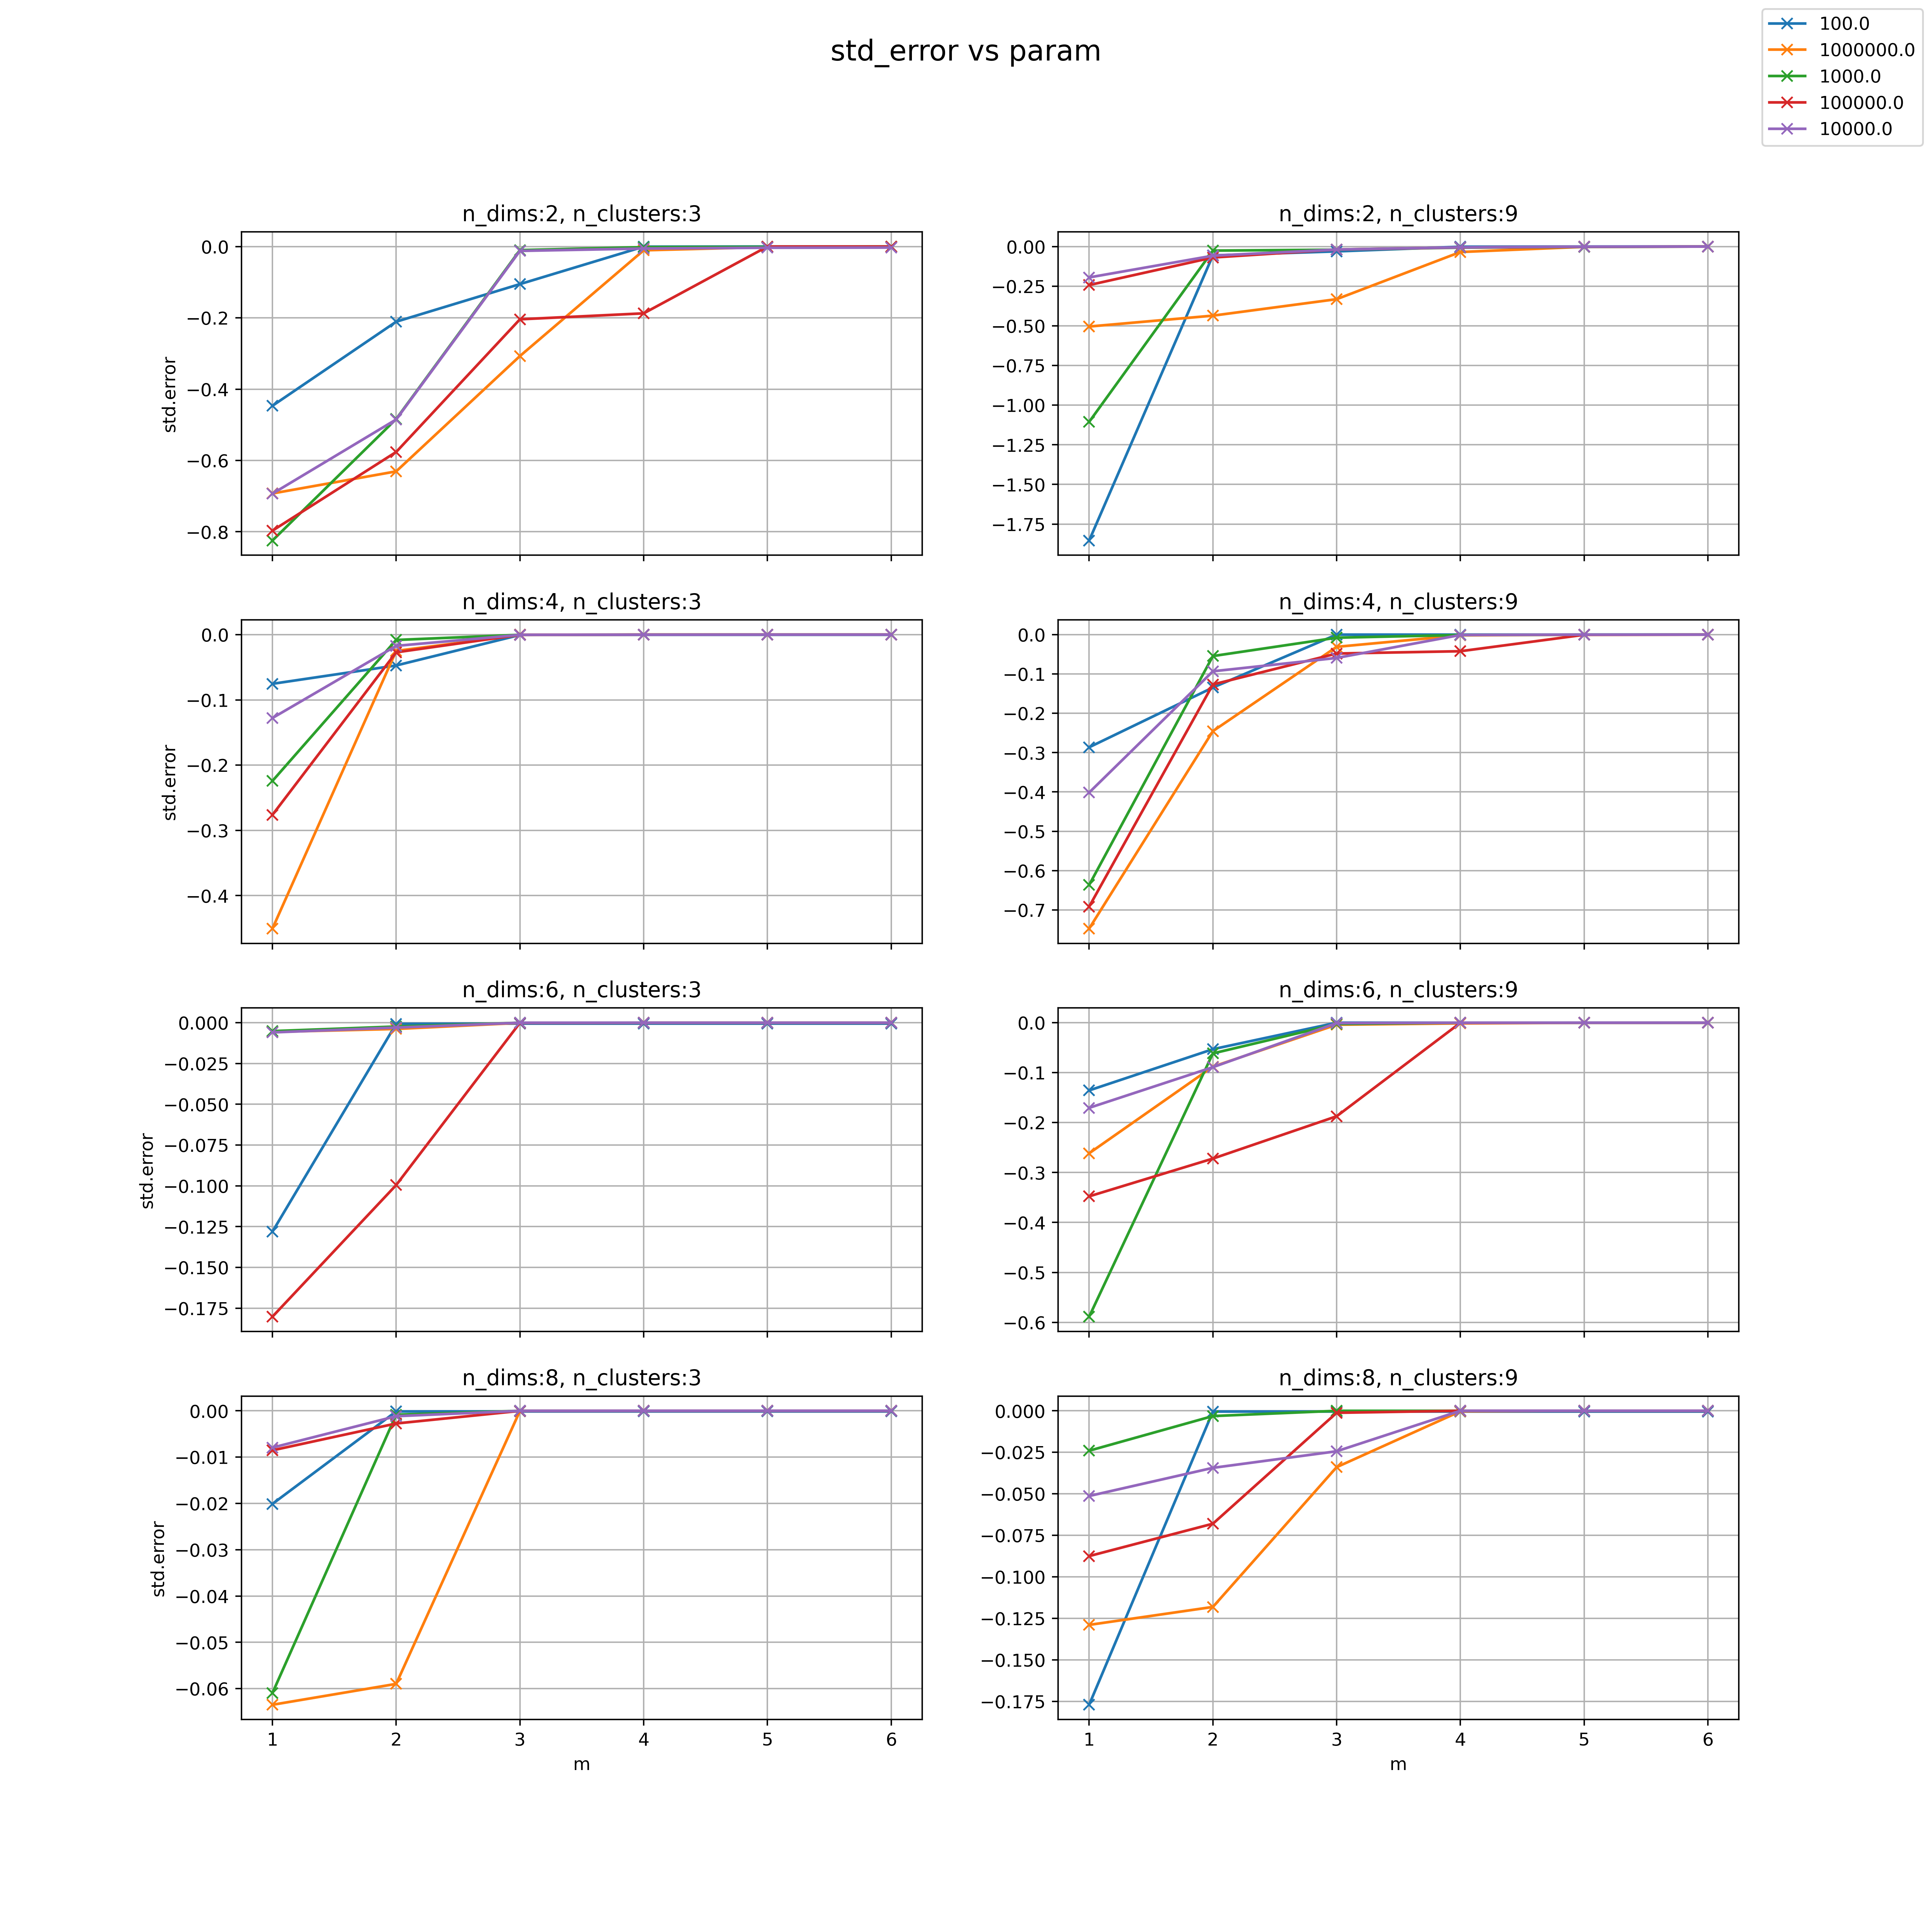
\includegraphics[width=\linewidth]{images/experiments/std_error_artificial.png}
    \caption{Standard error computation results in artificial datasets}
    \label{fig:error_art}
\end{figure}

\begin{figure}[!ht]
    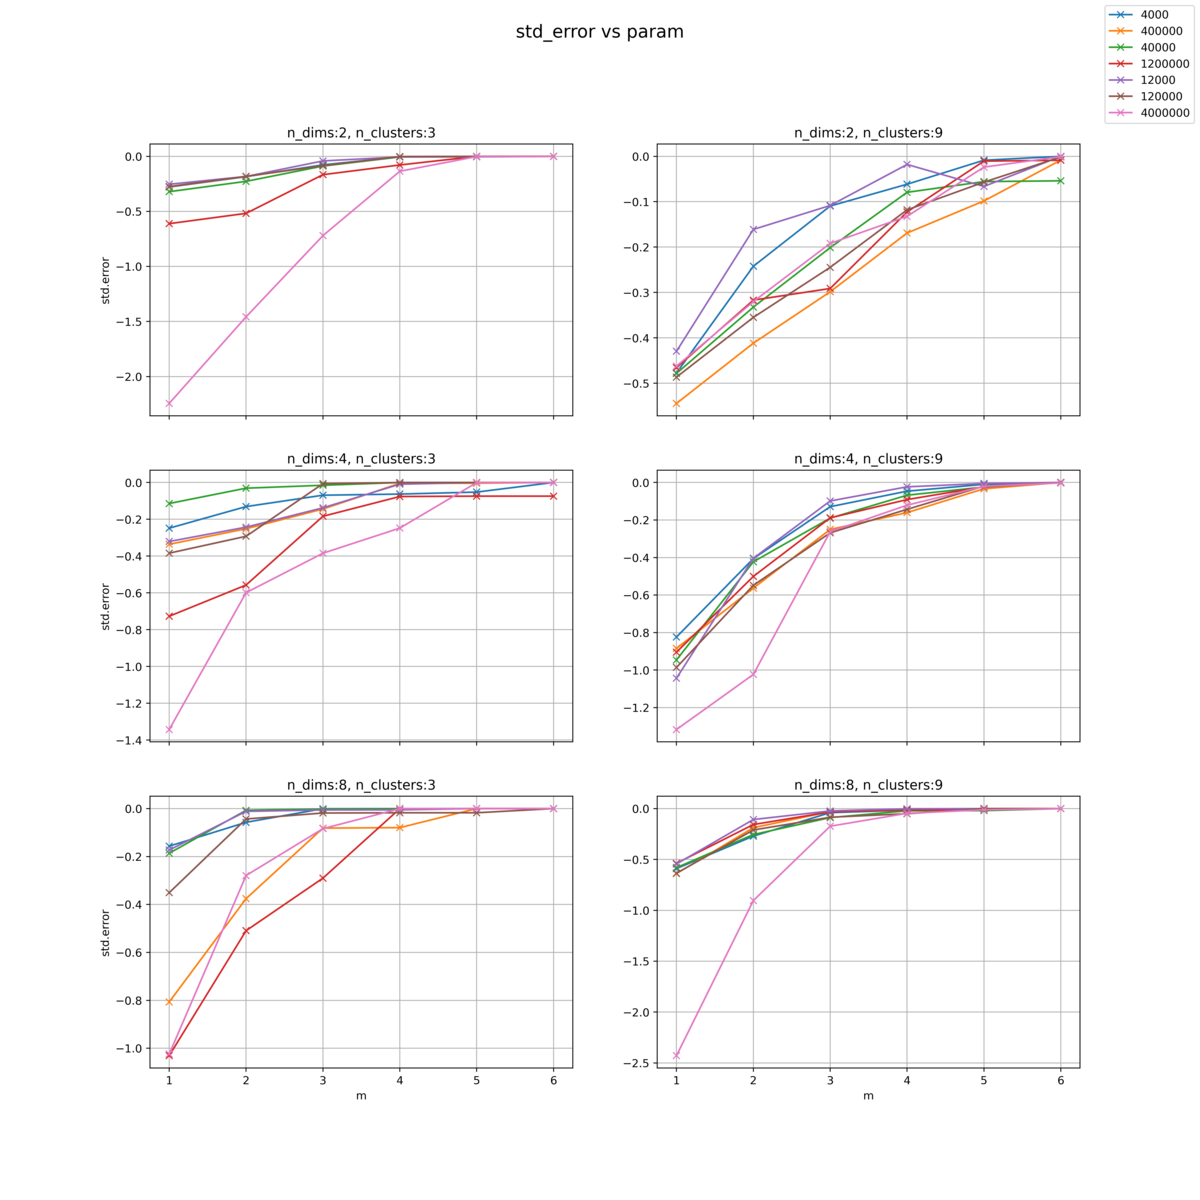
\includegraphics[width=\linewidth]{images/experiments/std_error_real.png}
    \caption{Standard error computation results in real datasets}
    \label{fig:error_real}
\end{figure}

From both figures we can extract the conclusion that the error decreases as $m$ increases and the number of representatives with it. The more clusters the error becomes more apparent wrt the k-means++ algorithm. Also as the number of dimensions increase, as the number of partitions increases the ratio approaches 1 and then the algorithm approximates very well the k-means++ error but by means of brute force.
